% REV00 Tue 04 May 2021 13:55:16 WIB
% START Tue 04 May 2021 13:55:16 WIB

\chapter{XXX}

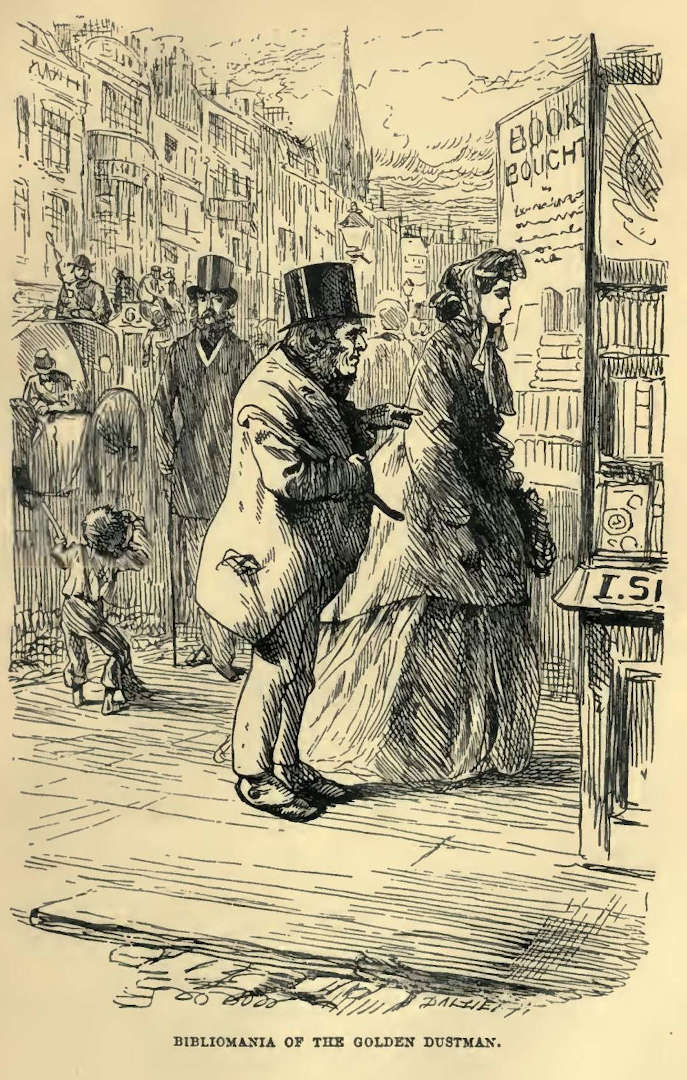
\includegraphics[scale=2.3]{03-05-01}

Chapter 14

CHECKMATE TO THE FRIENDLY MOVE


Mr and Mrs John Harmon had so timed their taking possession of their
rightful name and their London house, that the event befel on the very
day when the last waggon-load of the last Mound was driven out at the
gates of Boffin’s Bower. As it jolted away, Mr Wegg felt that the
last load was correspondingly removed from his mind, and hailed the
auspicious season when that black sheep, Boffin, was to be closely
sheared.

Over the whole slow process of levelling the Mounds, Silas had kept
watch with rapacious eyes. But, eyes no less rapacious had watched the
growth of the Mounds in years bygone, and had vigilantly sifted the dust
of which they were composed. No valuables turned up. How should there
be any, seeing that the old hard jailer of Harmony Jail had coined every
waif and stray into money, long before?

Though disappointed by this bare result, Mr Wegg felt too sensibly
relieved by the close of the labour, to grumble to any great extent.
A foreman-representative of the dust contractors, purchasers of the
Mounds, had worn Mr Wegg down to skin and bone. This supervisor of the
proceedings, asserting his employers’ rights to cart off by daylight,
nightlight, torchlight, when they would, must have been the death of
Silas if the work had lasted much longer. Seeming never to need sleep
himself, he would reappear, with a tied-up broken head, in fantail hat
and velveteen smalls, like an accursed goblin, at the most unholy and
untimely hours. Tired out by keeping close ward over a long day’s work
in fog and rain, Silas would have just crawled to bed and be dozing,
when a horrid shake and rumble under his pillow would announce an
approaching train of carts, escorted by this Demon of Unrest, to fall to
work again. At another time, he would be rumbled up out of his soundest
sleep, in the dead of the night; at another, would be kept at his post
eight-and-forty hours on end. The more his persecutor besought him not
to trouble himself to turn out, the more suspicious was the crafty Wegg
that indications had been observed of something hidden somewhere, and
that attempts were on foot to circumvent him. So continually broken was
his rest through these means, that he led the life of having wagered
to keep ten thousand dog-watches in ten thousand hours, and looked
piteously upon himself as always getting up and yet never going to bed.
So gaunt and haggard had he grown at last, that his wooden leg showed
disproportionate, and presented a thriving appearance in contrast
with the rest of his plagued body, which might almost have been termed
chubby.

However, Wegg’s comfort was, that all his disagreeables were now over,
and that he was immediately coming into his property. Of late, the
grindstone did undoubtedly appear to have been whirling at his own nose
rather than Boffin’s, but Boffin’s nose was now to be sharpened fine.
Thus far, Mr Wegg had let his dusty friend off lightly, having been
baulked in that amiable design of frequently dining with him, by the
machinations of the sleepless dustman. He had been constrained to depute
Mr Venus to keep their dusty friend, Boffin, under inspection, while he
himself turned lank and lean at the Bower.

To Mr Venus’s museum Mr Wegg repaired when at length the Mounds
were down and gone. It being evening, he found that gentleman, as he
expected, seated over his fire; but did not find him, as he expected,
floating his powerful mind in tea.

‘Why, you smell rather comfortable here!’ said Wegg, seeming to take it
ill, and stopping and sniffing as he entered.

‘I AM rather comfortable, sir,’ said Venus.

‘You don’t use lemon in your business, do you?’ asked Wegg, sniffing
again.

‘No, Mr Wegg,’ said Venus. ‘When I use it at all, I mostly use it in
cobblers’ punch.’

‘What do you call cobblers’ punch?’ demanded Wegg, in a worse humour
than before.

‘It’s difficult to impart the receipt for it, sir,’ returned Venus,
‘because, however particular you may be in allotting your materials,
so much will still depend upon the individual gifts, and there being a
feeling thrown into it. But the groundwork is gin.’

‘In a Dutch bottle?’ said Wegg gloomily, as he sat himself down.

‘Very good, sir, very good!’ cried Venus. ‘Will you partake, sir?’

‘Will I partake?’ returned Wegg very surlily. ‘Why, of course I will!
WILL a man partake, as has been tormented out of his five senses by
an everlasting dustman with his head tied up! WILL he, too! As if he
wouldn’t!’

‘Don’t let it put you out, Mr Wegg. You don’t seem in your usual
spirits.’

‘If you come to that, you don’t seem in your usual spirits,’ growled
Wegg. ‘You seem to be setting up for lively.’

This circumstance appeared, in his then state of mind, to give Mr Wegg
uncommon offence.

‘And you’ve been having your hair cut!’ said Wegg, missing the usual
dusty shock.

‘Yes, Mr Wegg. But don’t let that put you out, either.’

‘And I am blest if you ain’t getting fat!’ said Wegg, with culminating
discontent. ‘What are you going to do next?’

‘Well, Mr Wegg,’ said Venus, smiling in a sprightly manner, ‘I suspect
you could hardly guess what I am going to do next.’

‘I don’t want to guess,’ retorted Wegg. ‘All I’ve got to say is, that
it’s well for you that the diwision of labour has been what it has been.
It’s well for you to have had so light a part in this business, when
mine has been so heavy. You haven’t had YOUR rest broke, I’ll be bound.’

‘Not at all, sir,’ said Venus. ‘Never rested so well in all my life, I
thank you.’

‘Ah!’ grumbled Wegg, ‘you should have been me. If you had been me, and
had been fretted out of your bed, and your sleep, and your meals, and
your mind, for a stretch of months together, you’d have been out of
condition and out of sorts.’

‘Certainly, it has trained you down, Mr Wegg,’ said Venus, contemplating
his figure with an artist’s eye. ‘Trained you down very low, it has! So
weazen and yellow is the kivering upon your bones, that one might almost
fancy you had come to give a look-in upon the French gentleman in the
corner, instead of me.’

Mr Wegg, glancing in great dudgeon towards the French gentleman’s
corner, seemed to notice something new there, which induced him to
glance at the opposite corner, and then to put on his glasses and stare
at all the nooks and corners of the dim shop in succession.

‘Why, you’ve been having the place cleaned up!’ he exclaimed.

‘Yes, Mr Wegg. By the hand of adorable woman.’

‘Then what you’re going to do next, I suppose, is to get married?’

‘That’s it, sir.’

Silas took off his glasses again--finding himself too intensely
disgusted by the sprightly appearance of his friend and partner to bear
a magnified view of him and made the inquiry:

‘To the old party?’

‘Mr Wegg!’ said Venus, with a sudden flush of wrath. ‘The lady in
question is not a old party.’

‘I meant,’ exclaimed Wegg, testily, ‘to the party as formerly objected?’

‘Mr Wegg,’ said Venus, ‘in a case of so much delicacy, I must trouble
you to say what you mean. There are strings that must not be played
upon. No sir! Not sounded, unless in the most respectful and tuneful
manner. Of such melodious strings is Miss Pleasant Riderhood formed.’

‘Then it IS the lady as formerly objected?’ said Wegg.

‘Sir,’ returned Venus with dignity, ‘I accept the altered phrase. It is
the lady as formerly objected.’

‘When is it to come off?’ asked Silas.

‘Mr Wegg,’ said Venus, with another flush. ‘I cannot permit it to be
put in the form of a Fight. I must temperately but firmly call upon you,
sir, to amend that question.’

‘When is the lady,’ Wegg reluctantly demanded, constraining his ill
temper in remembrance of the partnership and its stock in trade, ‘a
going to give her ‘and where she has already given her ‘art?’

‘Sir,’ returned Venus, ‘I again accept the altered phrase, and with
pleasure. The lady is a going to give her ‘and where she has already
given her ‘art, next Monday.’

‘Then the lady’s objection has been met?’ said Silas.

‘Mr Wegg,’ said Venus, ‘as I did name to you, I think, on a former
occasion, if not on former occasions--’

‘On former occasions,’ interrupted Wegg.

‘--What,’ pursued Venus, ‘what the nature of the lady’s objection was, I
may impart, without violating any of the tender confidences since sprung
up between the lady and myself, how it has been met, through the kind
interference of two good friends of mine: one, previously acquainted
with the lady: and one, not. The pint was thrown out, sir, by those two
friends when they did me the great service of waiting on the lady to
try if a union betwixt the lady and me could not be brought to bear--the
pint, I say, was thrown out by them, sir, whether if, after marriage,
I confined myself to the articulation of men, children, and the lower
animals, it might not relieve the lady’s mind of her feeling respecting
being as a lady--regarded in a bony light. It was a happy thought, sir,
and it took root.’

‘It would seem, Mr Venus,’ observed Wegg, with a touch of distrust,
‘that you are flush of friends?’

‘Pretty well, sir,’ that gentleman answered, in a tone of placid
mystery. ‘So-so, sir. Pretty well.’

‘However,’ said Wegg, after eyeing him with another touch of distrust,
‘I wish you joy. One man spends his fortune in one way, and another in
another. You are going to try matrimony. I mean to try travelling.’

‘Indeed, Mr Wegg?’

‘Change of air, sea-scenery, and my natural rest, I hope may bring me
round after the persecutions I have undergone from the dustman with his
head tied up, which I just now mentioned. The tough job being ended and
the Mounds laid low, the hour is come for Boffin to stump up. Would ten
to-morrow morning suit you, partner, for finally bringing Boffin’s nose
to the grindstone?’

Ten to-morrow morning would quite suit Mr Venus for that excellent
purpose.

‘You have had him well under inspection, I hope?’ said Silas.

Mr Venus had had him under inspection pretty well every day.

‘Suppose you was just to step round to-night then, and give him orders
from me--I say from me, because he knows I won’t be played with--to be
ready with his papers, his accounts, and his cash, at that time in the
morning?’ said Wegg. ‘And as a matter of form, which will be agreeable
to your own feelings, before we go out (for I’ll walk with you part of
the way, though my leg gives under me with weariness), let’s have a look
at the stock in trade.’

Mr Venus produced it, and it was perfectly correct; Mr Venus undertook
to produce it again in the morning, and to keep tryst with Mr Wegg on
Boffin’s doorstep as the clock struck ten. At a certain point of the
road between Clerkenwell and Boffin’s house (Mr Wegg expressly insisted
that there should be no prefix to the Golden Dustman’s name) the
partners separated for the night.

It was a very bad night; to which succeeded a very bad morning. The
streets were so unusually slushy, muddy, and miserable, in the morning,
that Wegg rode to the scene of action; arguing that a man who was, as
it were, going to the Bank to draw out a handsome property, could well
afford that trifling expense.

Venus was punctual, and Wegg undertook to knock at the door, and conduct
the conference. Door knocked at. Door opened.

‘Boffin at home?’

The servant replied that MR Boffin was at home.

‘He’ll do,’ said Wegg, ‘though it ain’t what I call him.’

The servant inquired if they had any appointment?

‘Now, I tell you what, young fellow,’ said Wegg, ‘I won’t have it. This
won’t do for me. I don’t want menials. I want Boffin.’

They were shown into a waiting-room, where the all-powerful Wegg wore
his hat, and whistled, and with his forefinger stirred up a clock that
stood upon the chimneypiece, until he made it strike. In a few minutes
they were shown upstairs into what used to be Boffin’s room; which,
besides the door of entrance, had folding-doors in it, to make it one
of a suite of rooms when occasion required. Here, Boffin was seated at a
library-table, and here Mr Wegg, having imperiously motioned the servant
to withdraw, drew up a chair and seated himself, in his hat, close
beside him. Here, also, Mr Wegg instantly underwent the remarkable
experience of having his hat twitched off his head and thrown out of a
window, which was opened and shut for the purpose.

‘Be careful what insolent liberties you take in that gentleman’s
presence,’ said the owner of the hand which had done this, ‘or I will
throw you after it.’

Wegg involuntarily clapped his hand to his bare head, and stared at the
Secretary. For, it was he addressed him with a severe countenance, and
who had come in quietly by the folding-doors.

‘Oh!’ said Wegg, as soon as he recovered his suspended power of speech.
‘Very good! I gave directions for YOU to be dismissed. And you ain’t
gone, ain’t you? Oh! We’ll look into this presently. Very good!’

‘No, nor I ain’t gone,’ said another voice.

Somebody else had come in quietly by the folding-doors. Turning his
head, Wegg beheld his persecutor, the ever-wakeful dustman, accoutred
with fantail hat and velveteen smalls complete. Who, untying his
tied-up broken head, revealed a head that was whole, and a face that was
Sloppy’s.

‘Ha, ha, ha, gentlemen!’ roared Sloppy in a peal of laughter, and with
immeasureable relish. ‘He never thought as I could sleep standing, and
often done it when I turned for Mrs Higden! He never thought as I used
to give Mrs Higden the Police-news in different voices! But I did lead
him a life all through it, gentlemen, I hope I really and truly DID!’
Here, Mr Sloppy opening his mouth to a quite alarming extent, and
throwing back his head to peal again, revealed incalculable buttons.

‘Oh!’ said Wegg, slightly discomfited, but not much as yet: ‘one and one
is two not dismissed, is it? Bof--fin! Just let me ask a question. Who
set this chap on, in this dress, when the carting began? Who employed
this fellow?’

‘I say!’ remonstrated Sloppy, jerking his head forward. ‘No fellows, or
I’ll throw you out of winder!’

Mr Boffin appeased him with a wave of his hand, and said: ‘I employed
him, Wegg.’

‘Oh! You employed him, Boffin? Very good. Mr Venus, we raise our terms,
and we can’t do better than proceed to business. Bof--fin! I want the
room cleared of these two scum.’

‘That’s not going to be done, Wegg,’ replied Mr Boffin, sitting
composedly on the library-table, at one end, while the Secretary sat
composedly on it at the other.

‘Bof--fin! Not going to be done?’ repeated Wegg. ‘Not at your peril?’

‘No, Wegg,’ said Mr Boffin, shaking his head good-humouredly. ‘Not at my
peril, and not on any other terms.’

Wegg reflected a moment, and then said: ‘Mr Venus, will you be so good
as hand me over that same dockyment?’

‘Certainly, sir,’ replied Venus, handing it to him with much politeness.
‘There it is. Having now, sir, parted with it, I wish to make a small
observation: not so much because it is anyways necessary, or expresses
any new doctrine or discovery, as because it is a comfort to my mind.
Silas Wegg, you are a precious old rascal.’

Mr Wegg, who, as if anticipating a compliment, had been beating
time with the paper to the other’s politeness until this unexpected
conclusion came upon him, stopped rather abruptly.

‘Silas Wegg,’ said Venus, ‘know that I took the liberty of taking Mr
Boffin into our concern as a sleeping partner, at a very early period of
our firm’s existence.’

‘Quite true,’ added Mr Boffin; ‘and I tested Venus by making him a
pretended proposal or two; and I found him on the whole a very honest
man, Wegg.’

‘So Mr Boffin, in his indulgence, is pleased to say,’ Venus remarked:
‘though in the beginning of this dirt, my hands were not, for a few
hours, quite as clean as I could wish. But I hope I made early and full
amends.’

‘Venus, you did,’ said Mr Boffin. ‘Certainly, certainly, certainly.’

Venus inclined his head with respect and gratitude. ‘Thank you, sir.
I am much obliged to you, sir, for all. For your good opinion now, for
your way of receiving and encouraging me when I first put myself in
communication with you, and for the influence since so kindly brought
to bear upon a certain lady, both by yourself and by Mr John Harmon.’ To
whom, when thus making mention of him, he also bowed.

Wegg followed the name with sharp ears, and the action with sharp eyes,
and a certain cringing air was infusing itself into his bullying air,
when his attention was re-claimed by Venus.

‘Everything else between you and me, Mr Wegg,’ said Venus, ‘now explains
itself, and you can now make out, sir, without further words from me.
But totally to prevent any unpleasantness or mistake that might arise on
what I consider an important point, to be made quite clear at the close
of our acquaintance, I beg the leave of Mr Boffin and Mr John Harmon to
repeat an observation which I have already had the pleasure of bringing
under your notice. You are a precious old rascal!’

‘You are a fool,’ said Wegg, with a snap of his fingers, ‘and I’d have
got rid of you before now, if I could have struck out any way of doing
it. I have thought it over, I can tell you. You may go, and welcome. You
leave the more for me. Because, you know,’ said Wegg, dividing his next
observation between Mr Boffin and Mr Harmon, ‘I am worth my price, and
I mean to have it. This getting off is all very well in its way, and it
tells with such an anatomical Pump as this one,’ pointing out Mr Venus,
‘but it won’t do with a Man. I am here to be bought off, and I have
named my figure. Now, buy me, or leave me.’

‘I’ll leave you, Wegg,’ said Mr Boffin, laughing, ‘as far as I am
concerned.’

‘Bof--fin!’ replied Wegg, turning upon him with a severe air, ‘I
understand YOUR new-born boldness. I see the brass underneath YOUR
silver plating. YOU have got YOUR nose out of joint. Knowing that you’ve
nothing at stake, you can afford to come the independent game. Why,
you’re just so much smeary glass to see through, you know! But Mr Harmon
is in another sitiwation. What Mr Harmon risks, is quite another pair
of shoes. Now, I’ve heerd something lately about this being Mr
Harmon--I make out now, some hints that I’ve met on that subject in
the newspaper--and I drop you, Bof--fin, as beneath my notice. I ask Mr
Harmon whether he has any idea of the contents of this present paper?’

‘It is a will of my late father’s, of more recent date than the will
proved by Mr Boffin (address whom again, as you have addressed him
already, and I’ll knock you down), leaving the whole of his property
to the Crown,’ said John Harmon, with as much indifference as was
compatible with extreme sternness.

‘Bight you are!’ cried Wegg. ‘Then,’ screwing the weight of his body
upon his wooden leg, and screwing his wooden head very much on one side,
and screwing up one eye: ‘then, I put the question to you, what’s this
paper worth?’

‘Nothing,’ said John Harmon.

Wegg had repeated the word with a sneer, and was entering on some
sarcastic retort, when, to his boundless amazement, he found himself
gripped by the cravat; shaken until his teeth chattered; shoved back,
staggering, into a corner of the room; and pinned there.

‘You scoundrel!’ said John Harmon, whose seafaring hold was like that of
a vice.

‘You’re knocking my head against the wall,’ urged Silas faintly.

‘I mean to knock your head against the wall,’ returned John Harmon,
suiting his action to his words, with the heartiest good will; ‘and I’d
give a thousand pounds for leave to knock your brains out. Listen, you
scoundrel, and look at that Dutch bottle.’

Sloppy held it up, for his edification.

‘That Dutch bottle, scoundrel, contained the latest will of the many
wills made by my unhappy self-tormenting father. That will gives
everything absolutely to my noble benefactor and yours, Mr Boffin,
excluding and reviling me, and my sister (then already dead of a broken
heart), by name. That Dutch bottle was found by my noble benefactor and
yours, after he entered on possession of the estate. That Dutch bottle
distressed him beyond measure, because, though I and my sister were
both no more, it cast a slur upon our memory which he knew we had
done nothing in our miserable youth, to deserve. That Dutch bottle,
therefore, he buried in the Mound belonging to him, and there it lay
while you, you thankless wretch, were prodding and poking--often very
near it, I dare say. His intention was, that it should never see the
light; but he was afraid to destroy it, lest to destroy such a document,
even with his great generous motive, might be an offence at law. After
the discovery was made here who I was, Mr Boffin, still restless on the
subject, told me, upon certain conditions impossible for such a hound as
you to appreciate, the secret of that Dutch bottle. I urged upon him the
necessity of its being dug up, and the paper being legally produced and
established. The first thing you saw him do, and the second thing has
been done without your knowledge. Consequently, the paper now rattling
in your hand as I shake you--and I should like to shake the life out
of you--is worth less than the rotten cork of the Dutch bottle, do you
understand?’

Judging from the fallen countenance of Silas as his head wagged
backwards and forwards in a most uncomfortable manner, he did
understand.

‘Now, scoundrel,’ said John Harmon, taking another sailor-like turn on
his cravat and holding him in his corner at arms’ length, ‘I shall make
two more short speeches to you, because I hope they will torment you.
Your discovery was a genuine discovery (such as it was), for nobody had
thought of looking into that place. Neither did we know you had made it,
until Venus spoke to Mr Boffin, though I kept you under good observation
from my first appearance here, and though Sloppy has long made it
the chief occupation and delight of his life, to attend you like your
shadow. I tell you this, that you may know we knew enough of you to
persuade Mr Boffin to let us lead you on, deluded, to the last possible
moment, in order that your disappointment might be the heaviest possible
disappointment. That’s the first short speech, do you understand?’

Here, John Harmon assisted his comprehension with another shake.

‘Now, scoundrel,’ he pursued, ‘I am going to finish. You supposed me
just now, to be the possessor of my father’s property.--So I am. But
through any act of my father’s, or by any right I have? No. Through the
munificence of Mr Boffin. The conditions that he made with me, before
parting with the secret of the Dutch bottle, were, that I should take
the fortune, and that he should take his Mound and no more. I owe
everything I possess, solely to the disinterestedness, uprightness,
tenderness, goodness (there are no words to satisfy me) of Mr and Mrs
Boffin. And when, knowing what I knew, I saw such a mud-worm as you
presume to rise in this house against this noble soul, the wonder is,’
added John Harmon through his clenched teeth, and with a very ugly turn
indeed on Wegg’s cravat, ‘that I didn’t try to twist your head off,
and fling THAT out of window! So. That’s the last short speech, do you
understand?’

Silas, released, put his hand to his throat, cleared it, and looked as
if he had a rather large fishbone in that region. Simultaneously with
this action on his part in his corner, a singular, and on the surface
an incomprehensible, movement was made by Mr Sloppy: who began backing
towards Mr Wegg along the wall, in the manner of a porter or heaver who
is about to lift a sack of flour or coals.

‘I am sorry, Wegg,’ said Mr Boffin, in his clemency, ‘that my old lady
and I can’t have a better opinion of you than the bad one we are forced
to entertain. But I shouldn’t like to leave you, after all said and
done, worse off in life than I found you. Therefore say in a word,
before we part, what it’ll cost to set you up in another stall.’

‘And in another place,’ John Harmon struck in. ‘You don’t come outside
these windows.’

‘Mr Boffin,’ returned Wegg in avaricious humiliation: ‘when I first had
the honour of making your acquaintance, I had got together a collection
of ballads which was, I may say, above price.’

‘Then they can’t be paid for,’ said John Harmon, ‘and you had better not
try, my dear sir.’

‘Pardon me, Mr Boffin,’ resumed Wegg, with a malignant glance in the
last speaker’s direction, ‘I was putting the case to you, who, if my
senses did not deceive me, put the case to me. I had a very choice
collection of ballads, and there was a new stock of gingerbread in the
tin box. I say no more, but would rather leave it to you.’

‘But it’s difficult to name what’s right,’ said Mr Boffin uneasily, with
his hand in his pocket, ‘and I don’t want to go beyond what’s right,
because you really have turned out such a very bad fellow. So artful,
and so ungrateful you have been, Wegg; for when did I ever injure you?’

‘There was also,’ Mr Wegg went on, in a meditative manner, ‘a errand
connection, in which I was much respected. But I would not wish to be
deemed covetous, and I would rather leave it to you, Mr Boffin.’

‘Upon my word, I don’t know what to put it at,’ the Golden Dustman
muttered.

‘There was likewise,’ resumed Wegg, ‘a pair of trestles, for which alone
a Irish person, who was deemed a judge of trestles, offered five and
six--a sum I would not hear of, for I should have lost by it--and there
was a stool, a umbrella, a clothes-horse, and a tray. But I leave it to
you, Mr Boffin.’

The Golden Dustman seeming to be engaged in some abstruse calculation,
Mr Wegg assisted him with the following additional items.

‘There was, further, Miss Elizabeth, Master George, Aunt Jane, and Uncle
Parker. Ah! When a man thinks of the loss of such patronage as that;
when a man finds so fair a garden rooted up by pigs; he finds it hard
indeed, without going high, to work it into money. But I leave it wholly
to you, sir.’

Mr Sloppy still continued his singular, and on the surface his
incomprehensible, movement.

‘Leading on has been mentioned,’ said Wegg with a melancholy air, ‘and
it’s not easy to say how far the tone of my mind may have been lowered
by unwholesome reading on the subject of Misers, when you was leading me
and others on to think you one yourself, sir. All I can say is, that
I felt my tone of mind a lowering at the time. And how can a man put a
price upon his mind! There was likewise a hat just now. But I leave the
ole to you, Mr Boffin.’

‘Come!’ said Mr Boffin. ‘Here’s a couple of pound.’

‘In justice to myself, I couldn’t take it, sir.’

The words were but out of his mouth when John Harmon lifted his finger,
and Sloppy, who was now close to Wegg, backed to Wegg’s back, stooped,
grasped his coat collar behind with both hands, and deftly swung him
up like the sack of flour or coals before mentioned. A countenance of
special discontent and amazement Mr Wegg exhibited in this position,
with his buttons almost as prominently on view as Sloppy’s own, and
with his wooden leg in a highly unaccommodating state. But, not for many
seconds was his countenance visible in the room; for, Sloppy lightly
trotted out with him and trotted down the staircase, Mr Venus attending
to open the street door. Mr Sloppy’s instructions had been to deposit
his burden in the road; but, a scavenger’s cart happening to stand
unattended at the corner, with its little ladder planted against the
wheel, Mr S. found it impossible to resist the temptation of shooting Mr
Silas Wegg into the cart’s contents. A somewhat difficult feat, achieved
with great dexterity, and with a prodigious splash.



